\documentclass[5p,times,twocolumn]{elsarticle}

\usepackage[T1]{fontenc}
\usepackage[utf8]{inputenc}
\usepackage{amsmath,amssymb}
\usepackage{graphicx}
\usepackage{booktabs}
\usepackage{siunitx}
\usepackage[protrusion=true,expansion=true]{microtype}
\usepackage[hidelinks]{hyperref}
\usepackage{array}
\usepackage{tabularx}
\usepackage{float}

\sisetup{separate-uncertainty=true}
\graphicspath{{figures/}}
\newcommand{\familyone}{Classical Hall-Petch}
\newcommand{\familytwo}{Physics-derived descriptors}
\newcommand{\familythree}{Composition/processing}
\newcommand{\familyfour}{Non-linear ML (ARMOTE-CV)}
\newcommand{\familyfive}{Symbolic regression}
\renewcommand{\topfraction}{0.9}
\renewcommand{\bottomfraction}{0.8}
\renewcommand{\textfraction}{0.07}
\renewcommand{\floatpagefraction}{0.75}
\renewcommand{\dbltopfraction}{0.9}
\renewcommand{\dblfloatpagefraction}{0.75}
\setcounter{topnumber}{3}
\setcounter{dbltopnumber}{3}
\setcounter{totalnumber}{5}

\journal{Acta Materialia}

\begin{document}
\begin{frontmatter}

\title{Revisiting Hall-Petch strengthening in FCC Multi-principal element alloys: Best practices for building and auditing machine learning strength models}

\author[mse]{Mrinalini~Mulukutla\corref{cor1}}
\ead{mrinalini.mulukutla@tamu.edu}
\author[mae]{Shakti~Prasad~Padhy}
\author[mse]{Wenle~Xu}
\author[mse]{Bibhu~Prasad~Sahu}
\author[mse]{Joydeep~Kundu}
\author[mse]{Vasanth~C.~Shunmugasamy}
\author[mae]{Douglas~Allaire}
\author[mse]{Ibrahim~Karaman}
\author[mse,mae]{Raymundo~Arr\'{o}yave}
\cortext[cor1]{Corresponding author.}
\affiliation[mse]{organization={Department of Materials Science and Engineering, Texas A\&M University},
  city={College Station}, state={TX}, postcode={77843}, country={USA}}
\affiliation[mae]{organization={J. Mike Walker '66 Department of Mechanical Engineering, Texas A\&M University},
  city={College Station}, state={TX}, postcode={77843}, country={USA}}

\begin{abstract}
Machine-learning (ML) property models can mislead alloy design when interpolation is mistaken for transfer or physically motivated descriptors are interpreted as mechanisms without showing that they add information beyond the measured inputs. We present a best practices workflow that uses ML to build and audit physics-informed models of yield strength (YS) and Vickers hardness (HV) for 94 FCC multi-principal element alloy candidates. The dataset represents 82 unique compositions in the Al--Co--Cr--Cu--Fe--Mn--Ni--V system from two sequential closed-loop campaigns. Five fixed model families progress from \familyone{} through \familytwo, \familythree, \familyfour, and \familyfive. Comparisons use fold-contained preprocessing and pooled predictions from shuffled 5-fold, leave-one-out (LOO), and leave-one-batch-out (LOBO) validation, followed by a heterogeneous literature stress test and singularity audits of closed-form equations. For YS, the classical grain-size baseline gives LOO/LOBO $R^2=0.406/0.373$. The tested solid solution strengthening estimates add at most 0.002 in LOO $R^2$ once composition is present. A composition-dependent Hall--Petch intercept gives LOO/LOBO $R^2=0.652/0.625$. Adding grain-size standard deviation only as an additive term gives $0.668/0.595$, whereas allowing it to modify the Hall--Petch term gives $0.694/0.694$, the strongest verified low-complexity YS result. This improvement identifies a useful interaction within the sampled program, not an independent grain-width mechanism. At matched inputs, Lasso and LightGBM give similar YS LOBO scores (0.621 and 0.615), providing no evidence that non-linearity improves batch-level transfer. For HV, a post-selected symbolic fixed form gives LOO/LOBO $R^2=0.727/0.636$ after fold-wise coefficient refitting. The evaluated composition-dependent Hall--Petch and SISSO forms all have negative $R^2$ on the literature set of direct strength measurements. Increasing model flexibility therefore does not ensure transferable physics. Reliable property modeling requires a physical baseline, descriptor-redundancy tests, measured composition, processing, and microstructure before estimator complexity, external challenge data with explicit provenance, and equation-safety checks.
\end{abstract}

\begin{keyword}
Multi-principal element alloys \sep Hall--Petch \sep Machine learning \sep Symbolic regression \sep Grouped validation \sep Hardness
\end{keyword}
\end{frontmatter}

\section{Introduction}
\label{sec:intro}

Multi-principal element alloys (MPEAs) span composition and processing spaces that are high dimensional and too large to explore exhaustively~\cite{Cantor2004,Yeh2004,George2019,Miracle2017}. Closed-loop machine learning (ML) can speed up this search~\cite{Rao2022,Hastings2025FCC,Mulukutla2024BIRDSHOT,Mulukutla2026BRAVE}. However, a property model becomes harmful when a good interpolation score is used to support decisions about new compositions, processing routes, or experimental campaigns. This risk is especially high for small and sparse experimental datasets that represent these very high dimensional design spaces. Nearby compositions, repeated conditions, and campaign-specific processing can make a random train/test split much easier than the intended alloy design problem~\cite{Meredig2018,WangAYT2020,LiMDHIT2024}.

Yield strength offers a useful physical foundation. The Hall-Petch relation
\begin{equation}
\sigma_y=\sigma_0+k_{\mathrm{HP}}d^{-1/2}
\label{eq:hp}
\end{equation}
separates a grain-size-independent intercept from the grain-boundary strengthening term~\cite{Hall1951,Petch1953,Cordero2016}. In concentrated FCC alloys, composition can influence solid-solution resistance, ordering, stacking fault energy, and boundary-mediated deformation. Hall-Petch slopes and intercepts therefore vary significantly among alloy systems~\cite{Otto2013,Yoshida2017,LiKHP2024}. Several other grain-size laws can fit a limited range of $d$ almost as well as Eq.~\eqref{eq:hp}. A good regression fit alone therefore does not completely and accurately identify the underlying microscopic mechanism.

Physics-based solid solution strengthening (SSS) models and composition descriptors provide compact alternatives to using unconstrained elemental fractions~\cite{Varvenne2016,Varvenne2017,Labusch1970,TodaCaraballo2015,Wen2021SSS}. However, these descriptors are calculated directly from composition and may add little information after composition is already included. Non-linear and symbolic models can capture interactions that a linear model misses, but they also search a much larger space. As a result, they can exploit campaign identity, correlated descriptors, or unstable denominators. A feature can be physically meaningful without being transferable, and an equation can be interpretable without being a validated physical law.

Hardness serves as an additional, complementary target. Vickers hardness captures the material's resistance to deformation under localized loading. The empirical Tabor relation relates hardness to a representative flow stress, rather than directly to 0.2\% offset YS~\cite{Tabor1951,Dao2001}. Applying the same modeling and validation framework to YS and HV shows whether the relevant features depend on the property being modeled.

~\autoref{fig:framework} and Table~\ref{tab:families} define the five model families used throughout this paper, with the same names and order: Family~1 (\familyone), Family~2 (\familytwo), Family~3 (\familythree), Family~4 (\familyfour), and Family~5 (\familyfive). The families ask five sequential questions: What does grain size explain? Do physics-based descriptors capture the remaining strength? What do measured composition and processing add? Does non-linearity help when inputs are matched? Can symbolic search produce useful closed forms? A higher family number does not imply greater physical fidelity. We combine this hierarchy with 5-fold CV, record-level LOO, batch-level LOBO, an external literature stress test, and singularity auditing of closed-form equations.

\begin{table}[H]
\centering
\caption{Five model families used in the main paper and Supplementary Information.}
\label{tab:families}
\footnotesize
\begin{tabularx}{\columnwidth}{@{}c>{\raggedright\arraybackslash}p{2.70cm}>{\raggedright\arraybackslash}X@{}}
\toprule
Family & Fixed name & Analyses \\
\midrule
1 & \familyone & Classical and alternative grain-size laws \\
2 & \familytwo & SSS models, Wen descriptors, and PCA-OLS \\
3 & \familythree & OLS and composition-processing Hall--Petch models, including grain-width interactions \\
4 & \familyfour & Matched linear and non-linear estimators \\
5 & \familyfive & PySR, SISSO, and fixed closed forms \\
\bottomrule
\end{tabularx}
\end{table}


\begin{figure*}[t]
  \centering
  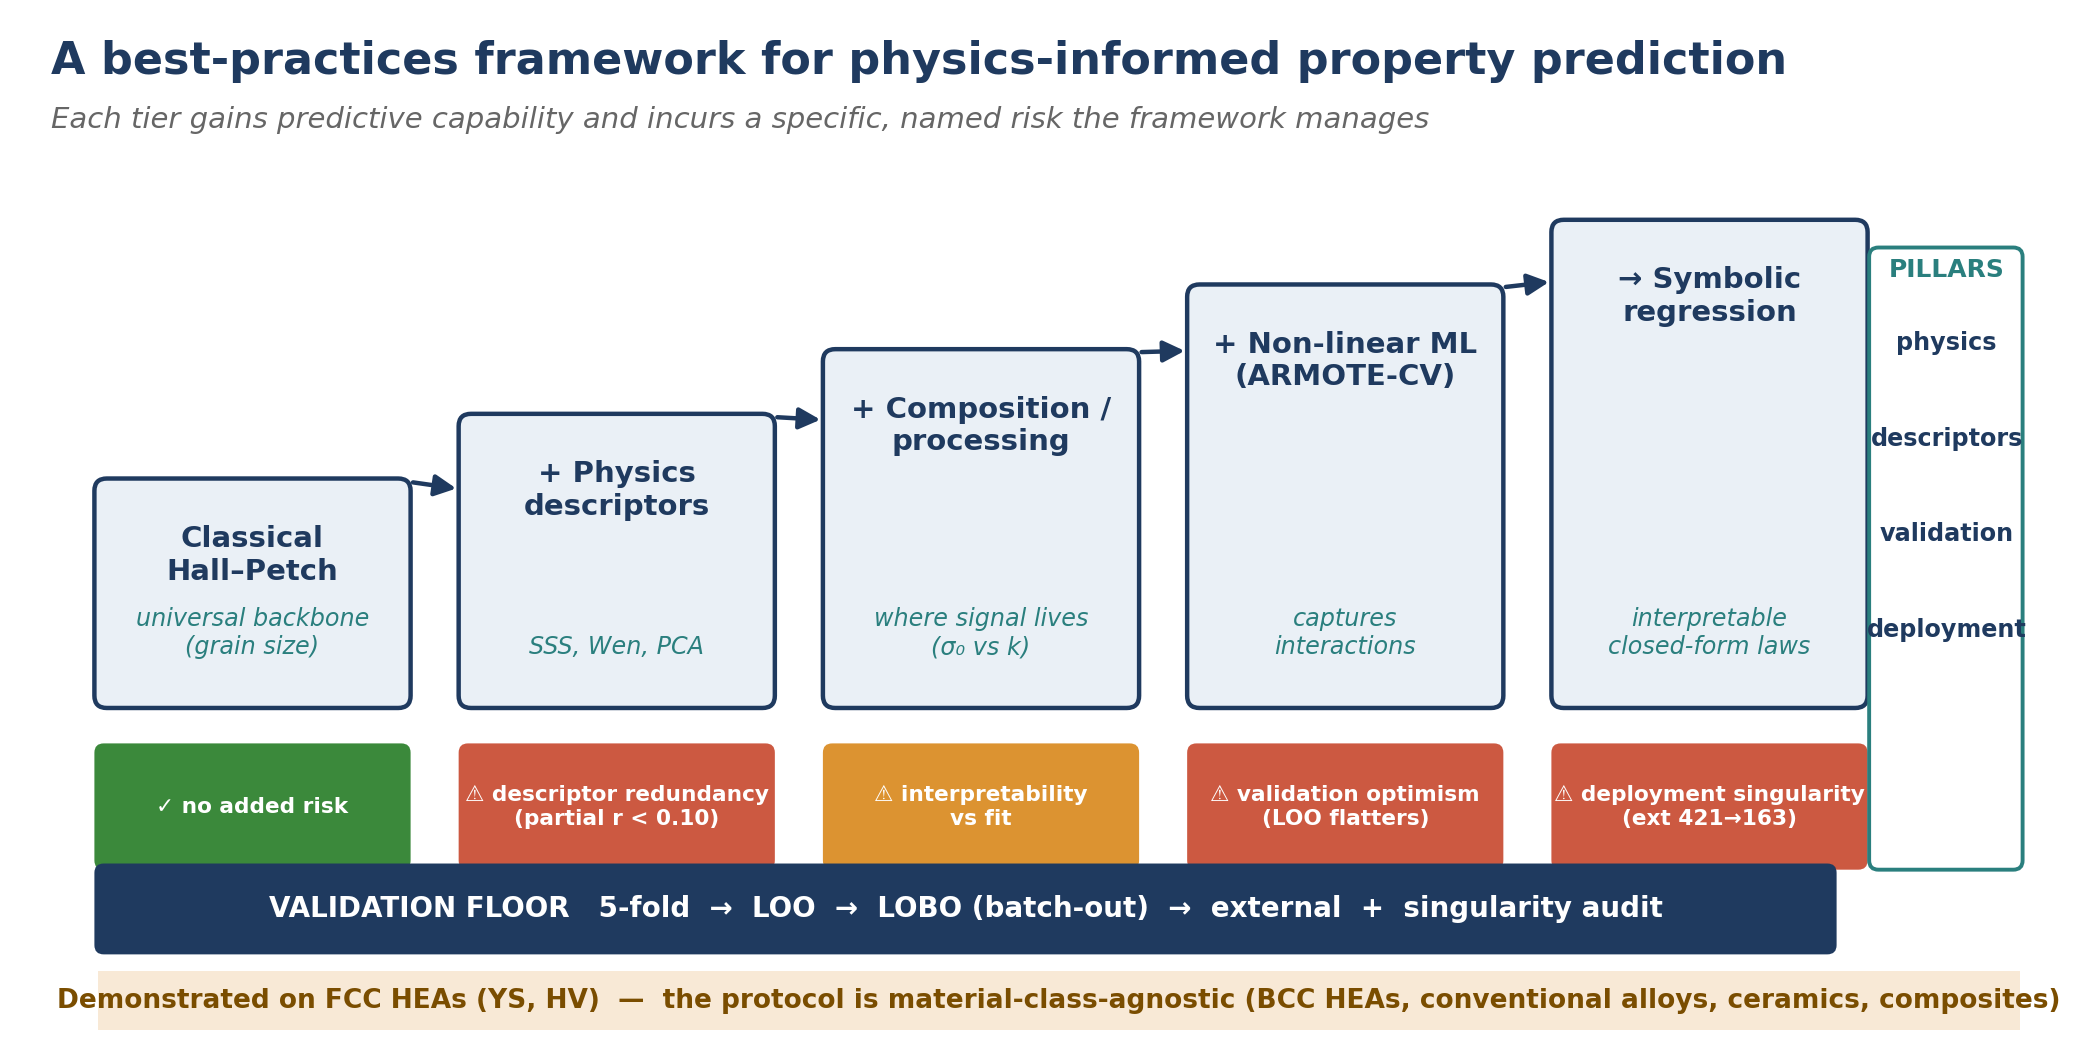
\includegraphics[width=0.9\textwidth]{fig00_framework_overview.png}
  \caption{Five family framework used throughout the paper: \familyone, \familytwo, \familythree, \familyfour, and \familyfive. S1--S4 name the matched input sets in Family~4; individual inputs, including $\mathrm{SD}_{\mathrm{grain}}$, are also tested in Families~2, 3, and 5. Internal evaluation uses 5-fold CV, LOO, and LOBO; external literature testing and singularity auditing provide additional challenge and equation safety checks.}
  \label{fig:framework}
\end{figure*}

\section{Dataset and descriptors}
\label{sec:data}

\subsection{Alloy Synthesis and characterization}

The dataset contains 94 FCC alloy conditions in the Al--Co--Cr--Cu--Fe--Mn--Ni--V system. YS is available for 93 conditions, and HV is available for all 94. An earlier Campaign A established the closed-loop, multi-objective alloy-discovery workflow used across this effort~\cite{Hastings2025FCC}; its records are not part of the present property-modeling dataset due to difference in the processing route for the same~\cite{Hastings2025FCC}. The samples analyzed here were generated from the subsequent B and C Bayesian optimization campaigns at Texas A\&M University within BIRDSHOT Center, supported by the U.S. Army DEVCOM High-Throughput Materials Discovery for Extreme Conditions (HTMDEC) initiative~\cite{Mulukutla2024BIRDSHOT,Mulukutla2026BRAVE}. The B campaign contributes 35 candidates from batches BBA, BBB, and BBC, including 34 with YS. It explored composition under an FCC phase stability constraint while holding processing fixed. The complete B-campaign synthesis and specimen preparation workflow is documented in Ref.~\cite{Mulukutla2026BRAVE}.

The C campaign contributes 59 candidates from CBA, CBB, and CBC. Building on the B-campaign results, it focused on a V--Cr--Mn--Fe--Co--Ni design space and jointly varied composition with three processing variables: cold work, recrystallization temperature, and hold time. Candidate alloys were iteratively selected from an FCC-constrained, manufacturable design space with the models updated after each iteration using the newly acquired data. A modified JMAK-type static-recrystallization and grain-growth prior supplied grain-size estimates over the feasible design space to guide candidate selection. That model and the complete C-campaign workflow will be reported in a separate future publication. The property models evaluated here use grain sizes measured by electron backscatter diffraction (EBSD), not these design-stage predictions.

Overall, both campaigns used the same high level production route: high-purity elemental feedstock was vacuum arc melted, homogenized, cold rolled, recrystallized, and quenched. Energy-dispersive X-ray spectroscopy (EDS) and X-ray diffraction were used to check realized chemistry and phase constitution, while electron microscopy and EBSD documented the microstructure. Grain size was measured from EBSD maps on surfaces normal to the rolling direction and summarized by the equivalent circle mean $d$ and within-map standard deviation $\mathrm{SD}_{\mathrm{grain}}$. Representative candidate alloy verification is shown in ~\autoref{fig:microstructure}. Quasistatic tensile testing was used to determine 0.2\% offset YS, while Vickers indentation tests provided the HV. Further details for BBA-BBC are given in Ref.~\cite{Mulukutla2026BRAVE}; a detailed account of CBA-CBC will follow in the campaign publication.

\begin{figure*}[t]
  \centering
  \includegraphics[width=0.7\textwidth]{composition_microstructure.png}
  \caption{Representative candidate alloy verification: measured and target composition, backscattered-electron imaging, an EBSD inverse-pole-figure map, and the corresponding equivalent-circle grain-size distribution. The right-skewed distribution motivates retaining both mean grain size and its within-map standard deviation.}
  \label{fig:microstructure}
\end{figure*}

\subsection{Coverage, dependence, and feature sets}

The 94 candidates in study represent 82 unique compositions: 73 chemistries occur once, and nine repeat across 21 records. Processing differs within eight of those nine groups, so these repeated chemistries capture grain size at fixed chemistry rather and varying processing condition; the exception is the CBB04/CBB12 pair, which shares both composition and processing (60\% cold work, \SI{875}{\degreeCelsius}, 1~h) and differs by \SI{32}{MPa} in YS and 4.7 in HV, the only direct estimate of repeatability the dataset contains. The 93-record YS subset contains 81
unique compositions. One composition appears in both CBB and CBC, so LOBO reduces campaign dependence without removing all exact-composition overlap, and LOO retains an identical chemistry in the training set for 21 of the 94 records. Mean $d$ ranges from 14.66 to \SI{211.75}{\micro\meter}, $\mathrm{SD}_{\mathrm{grain}}$ from 8.32 to \SI{321.06}{\micro\meter}, YS from 151.5 to \SI{544.5}{MPa}, and HV from 57.6 to 227.5. Because $d$ and $\mathrm{SD}_{\mathrm{grain}}$ are strongly correlated ($r=0.801$), we treat the standard deviation as an exploratory measure of distribution width rather than as an independent mechanism. Measurement scatter is a separate quantity: $\mathrm{SD}_{YS}$ is recorded for 80 conditions (0.2--\SI{98.7}{MPa}) and $\mathrm{SD}_{HV}$ for all 94 (1.43--12.44 HV). These measurement standard deviations are not model inputs because replicate counts and reporting definitions are not consistent across the dataset. The Bayesian optimization campaigns sample design-relevant regions, not a random composition simplex (~\autoref{fig:coverage}). 

\begin{figure*}[t]
  \centering
  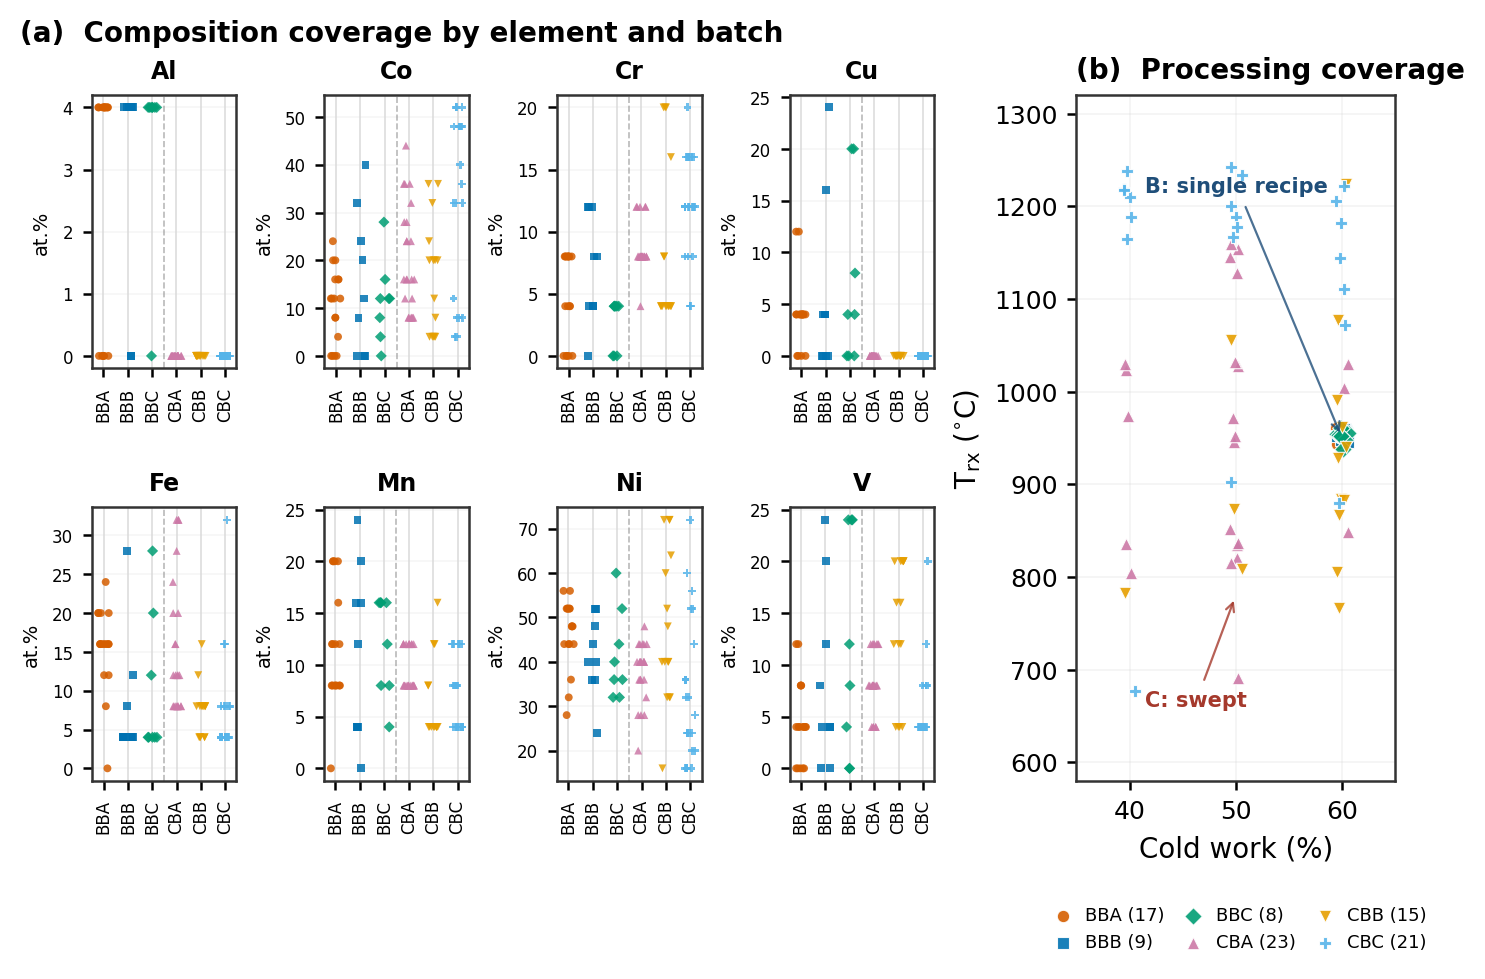
\includegraphics[width=0.92\textwidth]{fig_provenance.png}
  \caption{Composition and processing coverage by batch. The campaigns overlap but do not cover identical regions, and processing is partly structured by campaign. This data provenance motivates reporting LOBO along with record level validation instead of relying only on random splits.}
  \label{fig:coverage}
\end{figure*}

Table~\ref{tab:inputs} defines the cumulative S1-S4 input sets used for matched comparisons in Family~4. These labels refer to feature matrices, not model families. Raw composition is represented by eight atomic fractions when appropriate. Identifiable linear models use seven non-Ni fractions. The six Wen alloy descriptors are valence electron concentration (VEC), mixing enthalpy $\Delta H_{\mathrm{mix}}$, mixing entropy $\Delta S_{\mathrm{mix}}$, $\Omega$, electronegativity mismatch $\Delta\chi$, and atomic-size mismatch $\delta$~\cite{Wen2021SSS,Yang2012,Guo2011}.

\begin{table}[H]
\centering
\caption{Cumulative input sets used in Family~4.}
\label{tab:inputs}
\footnotesize
\begin{tabular}{@{}lcp{5.6cm}@{}}
\toprule
Set & $p$ & Content \\
\midrule
S1 & 2 & $d^{-1/2}$ and $\mathrm{SD}_{\mathrm{grain}}$ \\
S2 & 8 & S1 plus six Wen alloy descriptors \\
S3 & 11 & S2 plus cold work, $T_{\mathrm{rx}}$, and hold time \\
S4 & 24 & S3 plus composition and SSS-related quantities \\
\bottomrule
\end{tabular}
\end{table}


\section{Methods}
\label{sec:methods}

\subsection{Family 1: \familyone}

Equation~\eqref{eq:hp} provides the common grain-size baseline. We also compare nine pre-specified laws: $d^{-1/2}$, $d^{-1}$, $d^{-1/3}$, $d^{-2/3}$, $\ln(d)/d$, $\ln d$, two composite power-law forms, and a fitted free exponent. AIC, AICc, BIC, and Bayesian PSIS-LOO are used to compare these closely related parameterizations~\cite{Akaike1974,Schwarz1978,Vehtari2017,Yao2018}. We apply the same grain-size analysis separately to YS and HV.

\subsection{Family 2: \familytwo}

Family~2 tests whether compact physics-based representations explain YS and HV beyond the grain-size baseline. The Varvenne--Leyson--Curtin (VLC) model uses solute misfit volumes to estimate the zero temperature critical resolved shear stress,
\begin{equation}
\tau_{y0}=0.051\alpha^{-1/3}\bar\mu
\left(\frac{1+\bar\nu}{1-\bar\nu}\right)^{4/3}f_1
\left(\frac{\sum_i c_i\Delta V_i^2}{b^6}\right)^{2/3},
\label{eq:vlc}
\end{equation}
followed by a thermal activation correction and a Taylor factor. Here, $c_i$ and $\Delta V_i$ are the elemental fractions and misfit volumes, and $\bar\mu$, $\bar\nu$, and $b$ are composition averaged elastic and lattice quantities. Weighted Labusch and Toda-Caraballo estimates provide two related SSS representations. The Labusch and Toda-Caraballo constants are calibrated once to the reported CoCrFeMnNi friction stress; VLC is left uncalibrated. The full expressions and parameter values are given in the Supplementary Information.

These implementations use Vegard law volumes and rule-of-mixtures elastic properties~\cite{Varvenne2016,Varvenne2017,Labusch1970,TodaCaraballo2015}. We therefore keep calibrated and uncalibrated results separate. We also distinguish standalone prediction, improvement beyond Hall-Petch, and partial correlation after removing raw composition trends. These tests ask different questions, and partial correlation does not establish any form of independence.

The descriptor branch uses six Wen alloy descriptors together with $d^{-1/2}$, $\mathrm{SD}_{\mathrm{grain}}$, and three processing variables. Standardization and six-component PCA are fit again within each training fold before OLS. Full-data loadings are descriptive only. This fold-contained implementation corrects the preprocessing leakage in the earlier analysis.

\subsection{Family 3: \familythree}

Family~3 adds measured composition and processing to the Hall-Petch baseline through a pre-specified OLS hierarchy. Its principal model, M3, is
\begin{equation}
\sigma_y=\beta_0+\sum_{e\ne\mathrm{Ni}}\beta_e c_e
              +k_{\mathrm{HP}}d^{-1/2},
\label{eq:m3}
\end{equation}
where Ni is the composition reference. Other models allow only V in the intercept, composition-dependent slope terms, variation in both intercept and slope, descriptor substitutions, or recorded processing variables. The family name includes processing because the broader hierarchy tests those covariates, although M3 itself uses composition and $d$ without an explicit processing coefficient. Composition, processing, and grain size are interdependent in these campaigns. The fitted coefficients can therefore absorb covariance among them and are not interpreted as elemental constants.

The hierarchy is compared using information criteria and pooled out-of-fold predictions. We test $\mathrm{SD}_{\mathrm{grain}}$ first as an additive microstructure term and then through M15,
\begin{equation}
\sigma_y=\beta_0+\sum_{e\ne\mathrm{Ni}}\beta_e c_e
 +k_{\mathrm{HP}}d^{-1/2}+\gamma\mathrm{SD}_{\mathrm{grain}}
 +\eta\mathrm{SD}_{\mathrm{grain}}d^{-1/2}.
\label{eq:m15}
\end{equation}
The interaction allows the grain-distribution width to modify the fitted grain-size contribution. It is pre-specified OLS and can be reproduced from the prepared dataset, but its coefficients remain associational because $d$, $\mathrm{SD}_{\mathrm{grain}}$, composition, and processing are correlated.

\subsection{Family 4: \familyfour}

Family~4 compares linear controls and non-linear estimators using the same S1--S4 matrices and validation splits. OLS, Ridge, Lasso, and ElasticNet are retained so that the added value of non-linearity can be measured at fixed inputs. The primary audit uses declared, fixed parameter settings with no data-driven hyperparameter selection. For example, Lasso uses $\alpha=1.0$, while LightGBM uses 400 estimators, a maximum depth of 3, a learning rate of 0.05, and a feature fraction of 0.8. These are settings chosen for this study, not ``library defaults.'' An archived ARMOTE-CV table reports nested Optuna tuning for eight regressors. Because the repository does not contain its raw fold objects or generator, we use it only as secondary evidence. We also exclude the legacy full-data-tuned leaderboard from confirmatory rankings.

\subsection{Family 5: \familyfive}

PySR searches three feature pools and three operator sets, while SISSO provides a sparse operator comparison~\cite{Cranmer2023PySR,Ouyang2018SISSO}. PySR pool P1 contains grain statistics, P2 adds raw composition and processing, and P3 adds Wen descriptors and processing. The operator sets progress from addition and subtraction to multiplication, division, and protected non-linear operators. SISSO starts from 27 composition, thermodynamic, SSS, and grain-size features and builds two algebraic expansion levels before sparse selection.

In the stored workflow, equations were selected after the complete data search fronts had been viewed. Their constants were then refit within the CV folds. We therefore call these results ``post-selection fixed-form CV,'' rather than unbiased outer-loop estimates of symbolic discovery. Protected square root and logarithm are evaluated as $\sqrt{|x|}$ and $\log(|x|+\epsilon)$. We check each reported closed form for small or transformed denominators, sign changes, non-finite values, and extreme predictions over the observed internal and literature ranges. This audit is equation-specific and does not establish safety outside the stated descriptor envelope. BIC values from symbolic search are not compared directly with the pre-specified linear models because the stored symbolic parameter count omits the cost of searching variables, operators, and structures.

For HV, the selected structure is
\begin{equation}
H_V=c_0+c_1\frac{d_0-d}{\mathrm{SD}_{\mathrm{grain}}}
       +c_2\frac{\Delta H_{\mathrm{mix}}}{t_{\mathrm{hold}}^2}.
\label{eq:hvform}
\end{equation}
The constants are refit in every fold. In the reported equation, $d$, $d_0$, and $\mathrm{SD}_{\mathrm{grain}}$ are in \si{\micro\meter}, $t_{\mathrm{hold}}$ is in h, and $\Delta H_{\mathrm{mix}}$ is in kJ~mol$^{-1}$. Thus $c_0$ and $c_1$ have units of HV, while $c_2$ has units of HV$\cdot$h$^2\cdot$mol\,kJ$^{-1}$. This is an empirical expression, not a dimensionally universal relation. Its domain excludes $\mathrm{SD}_{\mathrm{grain}}\rightarrow0$ and $t_{\mathrm{hold}}\rightarrow0$.

\subsection{Validation hierarchy and score uncertainty}
\label{sec:validation}

We use three internal protocols that ask progressively different generalization questions: (i) shuffled 5-fold CV with seed 42; (ii) LOO; and (iii) LOBO across the six BO batches. LOO tests record-level interpolation, but another record with the same composition can remain in the training set. We therefore do not interpret LOO as strict new composition validation. LOBO tests transfer to a new iteration while retaining data from the broader experimental program and, in one case, the same composition.

For every protocol, predictions from all held-out records are pooled before computing
\begin{equation}
Q^2=1-\frac{\sum_i(y_i-\hat y_i)^2}{\sum_i(y_i-\bar y)^2}.
\end{equation}
We report this pooled quantity as cross-validated $R^2$. To calculate batch-clustered percentile intervals, we resample the six batches with replacement 1000 times while keeping every batch intact. These intervals show sensitivity to the sampled batches. With only six clusters, they should not be read as precise inferential confidence intervals. They quantify score uncertainty, not per-alloy predictive uncertainty; predictive intervals are outside the scope of this study.

The stored literature compilation has three evidence classes. E1 contains 54 direct strength records: 48 from the Borg/Citrine compilation~\cite{Borg2020} and six compression records for CrFeNi from Schneider and Laplanche~\cite{SchneiderCrFeNi2021}. These records represent only 18 exact compositions and mix sources and test modes. The legacy extraction limited grain size to 3--\SI{500}{\micro\meter}, removed YS values above \SI{800}{MPa}, and omitted one large-grain CrFeNi record because it departed from the expected Hall-Petch trend. Since two of these rules use the outcome or its expected relationship, we report E1 only as a heterogeneous literature stress test, not as an unbiased external validation set. E2 contains three values reconstructed from published Hall-Petch fits~\cite{Otto2013}. E3 contains 25 YS proxies converted from reported hardness~\cite{HuangTY2019}. We keep E2 and E3 separate from direct measurements.

For the hardness-strength comparison, hardness is converted to stress units and summarized as $C_{\mathrm{eff}}=\mathrm{HV(MPa)}/\sigma_y$. Under the conditional Tabor-Hollomon approximation,
\begin{equation}
n_{\mathrm{app}}=\frac{\ln(C_{\mathrm{eff}}/3)}{\ln(0.08/0.002)}
=\frac{\ln(C_{\mathrm{eff}}/3)}{\ln 40}.
\label{eq:napp}
\end{equation}
This is an apparent index, not a measured tensile hardening exponent, because offset YS is not the flow stress at exactly 0.002 true plastic strain and Hollomon behavior is assumed between 0.2\% and 8\% strain.

\section{Results}
\label{sec:results}

Table~\ref{tab:primary} gives the common comparison across model families. Five-fold CV and LOO mainly test interpolation within the pooled dataset, whereas LOBO asks whether a model transfers to an unseen experimental batch. We therefore base the main conclusions on LOBO together with the change from record-level to batch-level validation, rather than on the highest score in any one column. A negative $R^2$ means that the held-out predictions are worse than using the held-out mean.

\begin{table*}[t]
\centering
\caption{Pooled out-of-fold $R^2$ across the three internal validation protocols. LOBO provides the primary grouped transfer test. Family~4 includes linear controls to isolate the value of non-linearity. The Family~5 HV result is conditional on a structure selected using the full dataset.}
\label{tab:primary}
\footnotesize
\setlength{\tabcolsep}{3.8pt}
\begin{tabular}{lllrrr}
\toprule
Target & Family/model & Evidence status & 5-fold & LOO & LOBO \\
\midrule
YS & F1 Classical HP & baseline & 0.405 & 0.406 & 0.373 \\
YS & F2 PCA-OLS & fold-contained & 0.462 & 0.480 & 0.362 \\
YS & F3 M3 & pre-specified linear & 0.666 & 0.652 & 0.625 \\
YS & F3 M15 SD interaction & pre-specified linear & 0.731 & 0.694 & 0.694 \\
YS & F4 Lasso S2 & fixed settings & 0.683 & 0.674 & 0.621 \\
YS & F4 LightGBM S2 & fixed settings & 0.632 & 0.574 & 0.615 \\
HV & F1 Classical HP & baseline & 0.086 & 0.136 & $-0.077$ \\
HV & F4 LightGBM S1 & fixed settings & 0.195 & 0.323 & 0.112 \\
HV & F5 fixed form & post-selected & 0.725 & 0.727 & 0.636 \\
\bottomrule
\end{tabular}
\end{table*}

The grouped scores should also be read in light of composition coverage. Six principal components represent 96.9\% of the composition variance, and the mean pairwise batch-hull overlap in the PC1--PC2 projection is only about 0.21. CBC is relatively isolated in this projection, whereas CBA is well covered by the other batches. LOBO therefore combines easier interpolation-like folds with harder extrapolation folds; the pooled score is not a uniform measure of difficulty.

We do not report a single predictive ceiling. An in-sample composition-mean calculation gives $R^2\approx0.86$ if all 72 singleton compositions in the 93-record YS subset are assigned zero residual. In contrast, a calculation based only on repeated compositions gives a formal value near $-0.05$ because those groups also vary in processing and grain size. A separate estimate near 0.97 treats reported within-alloy standard deviations as irreducible target error, but replicate counts are unavailable. None of these quantities is a defensible out-of-sample ceiling.

\subsection{Family 1: \familyone}

The classical Hall--Petch law provides the grain-size-only baseline. For YS, it gives training $R^2=0.429$, LOO $R^2=0.406$ with RMSE $=\SI{62.5}{MPa}$, and LOBO $R^2=0.373$ (Fig.~\ref{fig:hp}). Its similar LOO and LOBO scores show that mean grain size contains a modest, reproducible YS signal.

The exact grain-size law is less certain. Nine pre-specified forms were compared. Five two-parameter monotonic laws lie within $\Delta\mathrm{BIC}<2$ and have LOO $R^2$ from 0.395 to 0.406. The free-exponent fit gives $n=0.548$, but its additional parameter raises $\Delta\mathrm{BIC}$ to 4.5. The Bayesian estimate is $n=0.53\pm0.16$, with a 94\% highest-density interval of about $[0.22,0.82]$. Bayesian stacking places all weight on the classical form, but the candidate laws have nearly equal expected log predictive density, so this boundary weight is not decisive. The data support $d^{-1/2}$ as a simple baseline, not as a uniquely identified exponent or mechanism.

The same baseline does not describe HV well. The classical form has training/LOO $R^2=0.169/0.136$ and becomes negative under LOBO ($-0.077$). A full-data optimized exponent of 1.728 raises LOO $R^2$ only to 0.166 and is descriptive because the exponent was selected before CV. Mean grain size alone therefore does not transfer as a hardness model.

\begin{figure}[t]
  \centering
  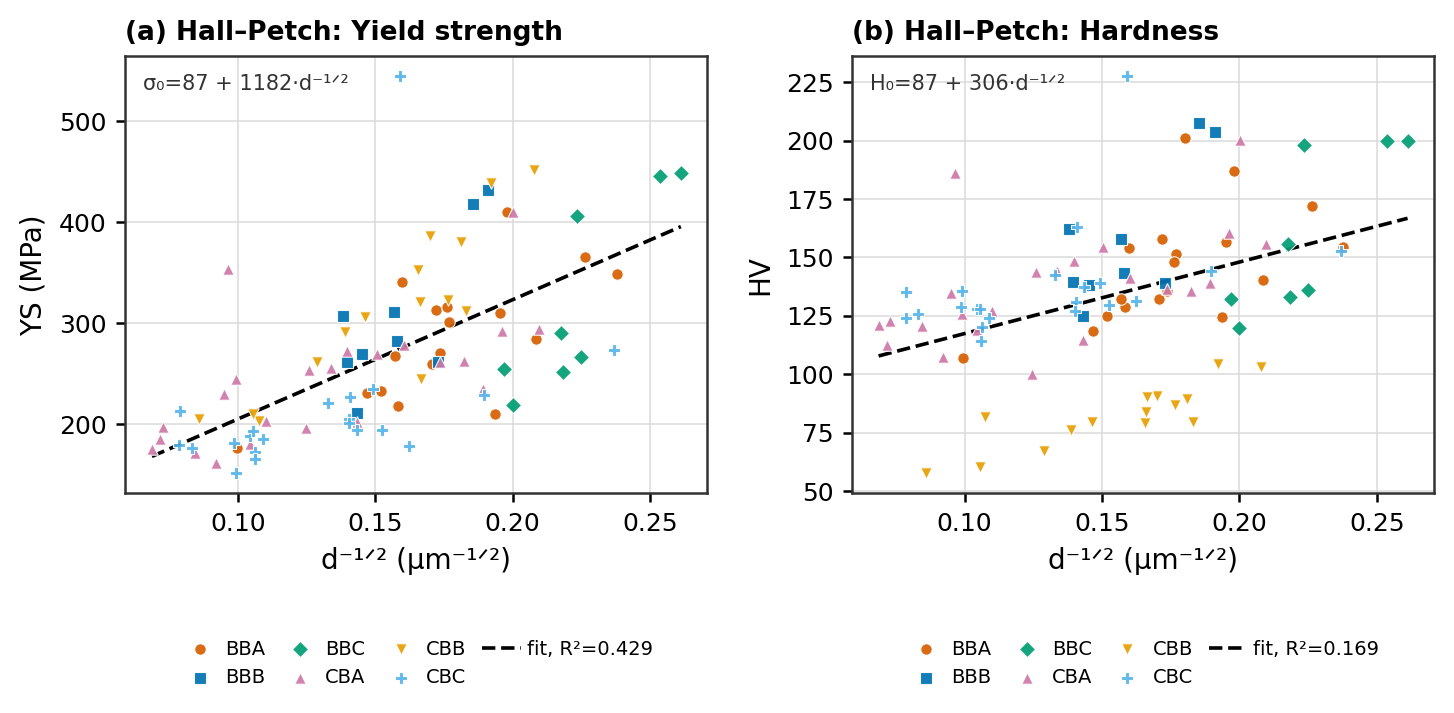
\includegraphics[width=\columnwidth]{fig01_hall_petch.png}
  \caption{Family~1 \familyone{} fits for YS and HV. Grain size provides a useful baseline for YS, but mean grain size alone does not transfer for HV.}
  \label{fig:hp}
\end{figure}

\subsection{Family 2: \familytwo}

Family~2 tests whether physics-derived descriptors add information beyond grain size and composition. For the SSS estimates, Cantor-anchored Labusch calibration gives a mean prediction-to-observation ratio of 1.07. Calibrated Toda--Caraballo and VLC overpredict by 42\% and 78\%, and uncalibrated variants overpredict by factors of 2--5. Used alone, VLC, Labusch, and Toda--Caraballo give LOO $R^2=0.030$, 0.274, and 0.091. Adding $d^{-1/2}$ changes these values to 0.396, 0.469, and 0.399, compared with 0.406 for Hall--Petch alone (Table~\ref{tab:sss-main}). Only calibrated Labusch gives a small improvement over that baseline (Fig.~\ref{fig:sss}).

The descriptors do not add information once composition is included. Adding an SSS estimate to a composition model changes LOO $R^2$ by at most 0.002, and all linear partial correlations after removing composition are below 0.10 in magnitude. This redundancy applies to the present descriptor inputs; it does not distinguish limitations of SSS theory from uncertainty in atomic volumes, elastic properties, calibration, or unmeasured microstructure.

The broader Wen/PCA representation gives 5-fold/LOO/LOBO $R^2=0.462/0.480/0.362$ when PCA is fitted inside each fold. Global preprocessing had produced 0.525/0.516/0.441, showing that even unsupervised scaling and PCA can inflate held-out scores when fitted before the split. The corrected LOBO result is below the classical Hall--Petch baseline, so the PCA model does not provide a transferable improvement at the batch level. Full-data loadings are therefore used only to describe the descriptor space, not as causal feature importance.

\begin{table*}[t]
\centering
\caption{Family~2 YS descriptor results. Ratio is mean SSS prediction divided by mean Hall--Petch-corrected YS. Raw $R^2$ and Spearman $\rho$ compare the complete-data SSS estimates with the corrected YS. Standalone and $+$HP are LOO results; $+$HP is Ridge using the SSS estimate and $d^{-1/2}$.}
\label{tab:sss-main}
\footnotesize
\setlength{\tabcolsep}{4pt}
\begin{tabular}{lrrrrrrr}
\toprule
Model & Mean (MPa) & Ratio & Raw $R^2$ & Spearman $\rho$ & Standalone $R^2$ & $+$HP $R^2$ & $+$HP RMSE (MPa) \\
\midrule
VLC & 342 & 1.78 & $-6.92$ & 0.53 & 0.030 & 0.396 & 63.1 \\
Labusch, calibrated & 206 & 1.07 & 0.14 & 0.55 & 0.274 & 0.469 & 59.1 \\
Toda--Caraballo, calibrated & 274 & 1.42 & $-3.18$ & 0.49 & 0.091 & 0.399 & 62.9 \\
HP only & --- & --- & --- & --- & --- & 0.406 & 62.5 \\
\bottomrule
\end{tabular}
\end{table*}

\begin{figure}[t]
  \centering
  
\includegraphics[width=0.88\columnwidth]{fig_sss_parity.png}
  \caption{Family~2 SSS predictions compared with Hall--Petch-corrected YS. Calibration can reduce average bias without showing that the descriptor transfers or adds information beyond composition.}
  \label{fig:sss}
\end{figure}

\subsection{Family 3: \familythree}

Family~3 adds composition, processing, and measured microstructure terms to the Hall--Petch baseline. M3 gives LOO/LOBO $R^2=0.652/0.625$ and LOBO RMSE $=\SI{49.7}{MPa}$. Its batch-bootstrap interval for LOBO $R^2$ is $[0.501,0.670]$, while the six individual batch-held-out scores range from 0.306 to 0.697. This spread shows that transfer difficulty differs across batches. M3 therefore retains useful YS information beyond mean grain size across the sampled experimental iterations.

The grain-size distribution adds information only in a specific form (Fig.~\ref{fig:mmodel}). Adding $\mathrm{SD}_{\mathrm{grain}}$ to M3 as an independent linear term raises LOO $R^2$ from 0.652 to 0.668 but lowers LOBO from 0.625 to 0.595. M15, which includes both the additive term and $\mathrm{SD}_{\mathrm{grain}}d^{-1/2}$, gives 5-fold/LOO/LOBO $R^2=0.731/0.694/0.694$ and LOBO RMSE $=\SI{44.9}{MPa}$. Its LOO and LOBO batch-bootstrap intervals are $[0.578,0.766]$ and $[0.599,0.733]$. Relative to M3, M15 lowers BIC by 20.1; the interaction coefficient has $t=4.71$ ($p=1.0\times10^{-5}$) in the complete-data OLS fit. M15 is therefore the strongest verified low-complexity YS model when $\mathrm{SD}_{\mathrm{grain}}$ is measured. The additive control shows that the gain cannot be credited to grain-width measurement alone. Because the term is correlated with mean grain size and processing, it is interpreted as a predictive interaction, not as proof that distribution width changes the Hall--Petch slope.

The individual M3 LOBO scores are 0.697 for BBA, 0.306 for BBB, 0.656 for BBC, 0.423 for CBA, 0.584 for CBB, and 0.409 for CBC; the corresponding RMSE values range from 32.9 to \SI{60.4}{MPa}. CBC has the lowest projected hull containment (0.476), while CBA has complete containment in the PC1--PC2 projection. Coverage is not the only source of error, but these folds show why the pooled LOBO score should be accompanied by batch-level results.

The complete-data M3 fit gives $k_{\mathrm{HP}}=766$~MPa$\cdot\mu$m$^{1/2}$. Adding the composition-dependent intercept lowers the slope from about 1149~MPa$\cdot\mu$m$^{1/2}$ in the grain-only fit, consistent with composition--grain-size confounding in Family~1. The M3 value is higher than several representative directly reported values, which span 110--538~MPa$\cdot\mu$m$^{1/2}$ in the cited pure metals and FCC MPEAs~\cite{Cordero2016,Yoshida2017,Otto2013,Yoshida2019acta}. This comparison is not an exhaustive literature bound, and the fitted M3 value should not be treated as a universal FCC value. Among the composition coefficients (Table~\ref{tab:m3-main}), V is the largest positive term relative to Ni ($+291$~MPa), but all coefficients are conditional on the sampled compositions and processing routes.

Two sensitivity checks address numerical stability of this fit. Across 1000 grain-size perturbations, the V, Co, Cr, and Fe coefficients change by less than about 15\%, whereas $k_{\mathrm{HP}}$ changes by about 39\%. Al is not included in the 15\% statement because it spans only 0--4~at.\% and has a much wider interval. A 10,000-replicate row bootstrap gives standard-error ratios of 0.99--1.54 relative to OLS. These checks support stability within the sampled records, but a row bootstrap does not reproduce campaign-level sampling and cannot establish transfer.

\begin{table}[t]
\centering
\caption{Family~3 M3 coefficients relative to Ni. Intervals are conditional on the OLS specification and sampled campaigns.}
\label{tab:m3-main}
\footnotesize
\begin{tabular}{lrrr}
\toprule
Parameter & Estimate (MPa) & 95\% low & 95\% high \\
\midrule
Intercept & 229.6 & 152.4 & 306.7 \\
Al & $-201.3$ & $-955.4$ & 552.8 \\
Co & $-187.2$ & $-268.1$ & $-106.3$ \\
Cr & $-307.7$ & $-588.5$ & $-26.9$ \\
Cu & $-334.0$ & $-651.9$ & $-16.2$ \\
Fe & $-360.4$ & $-520.1$ & $-200.6$ \\
Mn & 82.3 & $-117.6$ & 282.2 \\
V & 291.3 & 41.0 & 541.5 \\
$k_{\mathrm{HP}}$ & 765.8 & 501.5 & 1030.0 \\
\bottomrule
\end{tabular}
\end{table}

M3 assumes a shared Hall--Petch slope, but the dataset cannot test that assumption decisively. Only nine compositions are repeated, most have two records, and processing changes within some groups. Their descriptive local slopes range from about $-8539$ to 9282~MPa$\cdot\mu$m$^{1/2}$. A fixed-effect summary gives a slope near 2144, Cochran $Q\approx251$, and $I^2=96.8\%$, but this apparent heterogeneity cannot be assigned to composition under the present design. The data therefore do not show that $k_{\mathrm{HP}}$ is composition-independent. The supported result is narrower: a composition-dependent intercept with a shared grain-size term predicts YS well across the sampled batches. The physical division among friction stress, processing, and grain-boundary strengthening remains unresolved.

\begin{figure*}[t]
  \centering
  
\includegraphics[width=0.86\textwidth]{fig_comp_hp_models_ab.png}
  \caption{Family~3 Hall--Petch hierarchy for YS. M15 adds $\mathrm{SD}_{\mathrm{grain}}$ to M3 both directly and through the interaction $\mathrm{SD}_{\mathrm{grain}}d^{-1/2}$. It gives the strongest internal result, but its coefficients remain conditional on the sampled campaigns and correlated microstructure.}
  \label{fig:mmodel}
\end{figure*}

\subsection{Family 4: \familyfour}

Family~4 tests whether non-linear estimators improve prediction when the input set is held fixed. At S2, Lasso and LightGBM give nearly identical YS LOBO scores of 0.621 and 0.615. Their batch-bootstrap intervals also overlap: $[0.516,0.664]$ for Lasso and $[0.474,0.664]$ for LightGBM. This does not prove statistical equivalence, but it gives no evidence that non-linearity improves batch-level transfer at matched inputs. At S1, adding $\mathrm{SD}_{\mathrm{grain}}$ to the linear YS grain-size baseline changes LOO/LOBO $R^2$ from $0.406/0.373$ to $0.451/0.394$, a small gain that is much weaker than the M15 interaction result.

The archived nested ARMOTE-CV summary reports Bayesian ridge at S2 with 5-fold/LOO/LOBO $R^2=0.685/0.666/0.613$, which supports the same interpretation. The repository does not contain its generator or raw fold objects, and the available script tunes once on the full dataset. We therefore retain this result as secondary evidence rather than presenting it as independently reproduced nested CV.

The legacy 17-model panel gives a useful warning about model selection. Its XGBoost model reached LOO/LOBO $R^2=0.729/0.574$ after tuning and interaction construction on the complete dataset. Those values are not used in the primary ranking. The archived SHAP analysis explains that fitted model, but correlated descriptors and constructed interactions prevent causal interpretation of its feature rankings.

The same panel reported stacking LOBO $R^2=0.707$, but its meta-features were record-level LOO predictions from models that could retain other records from the held-out batch. This leakage prevents a grouped-transfer interpretation. In the fitted XGBoost model, SHAP ranks $\Omega$, Mn$\times d^{-1}$, V$\times d^{-1}$, alternative grain-size transforms, and SSS descriptors highly. These attributions describe the selected predictor; they do not isolate mechanisms or prove a composition-dependent Hall--Petch slope.

For HV, the Family~4 S1 matrix contains both $d^{-1/2}$ and $\mathrm{SD}_{\mathrm{grain}}$, whereas the Family~1 baseline contains only $d^{-1/2}$. With a linear estimator, this added feature changes LOO/LOBO $R^2$ from $0.136/-0.077$ to $0.232/-0.176$: it improves record-level interpolation but worsens batch transfer. LightGBM on S1 gives $0.323/0.112$. The comparison therefore changes both the feature set and estimator, and the LOO gain cannot be credited entirely to non-linearity. Descriptor-rich Family~4 input sets are generally negative under LOBO (Fig.~\ref{fig:fair}). The model can interpolate among related records, but it provides little evidence of reliable transfer to an unseen experimental batch.

\begin{figure}[t]
  \centering
  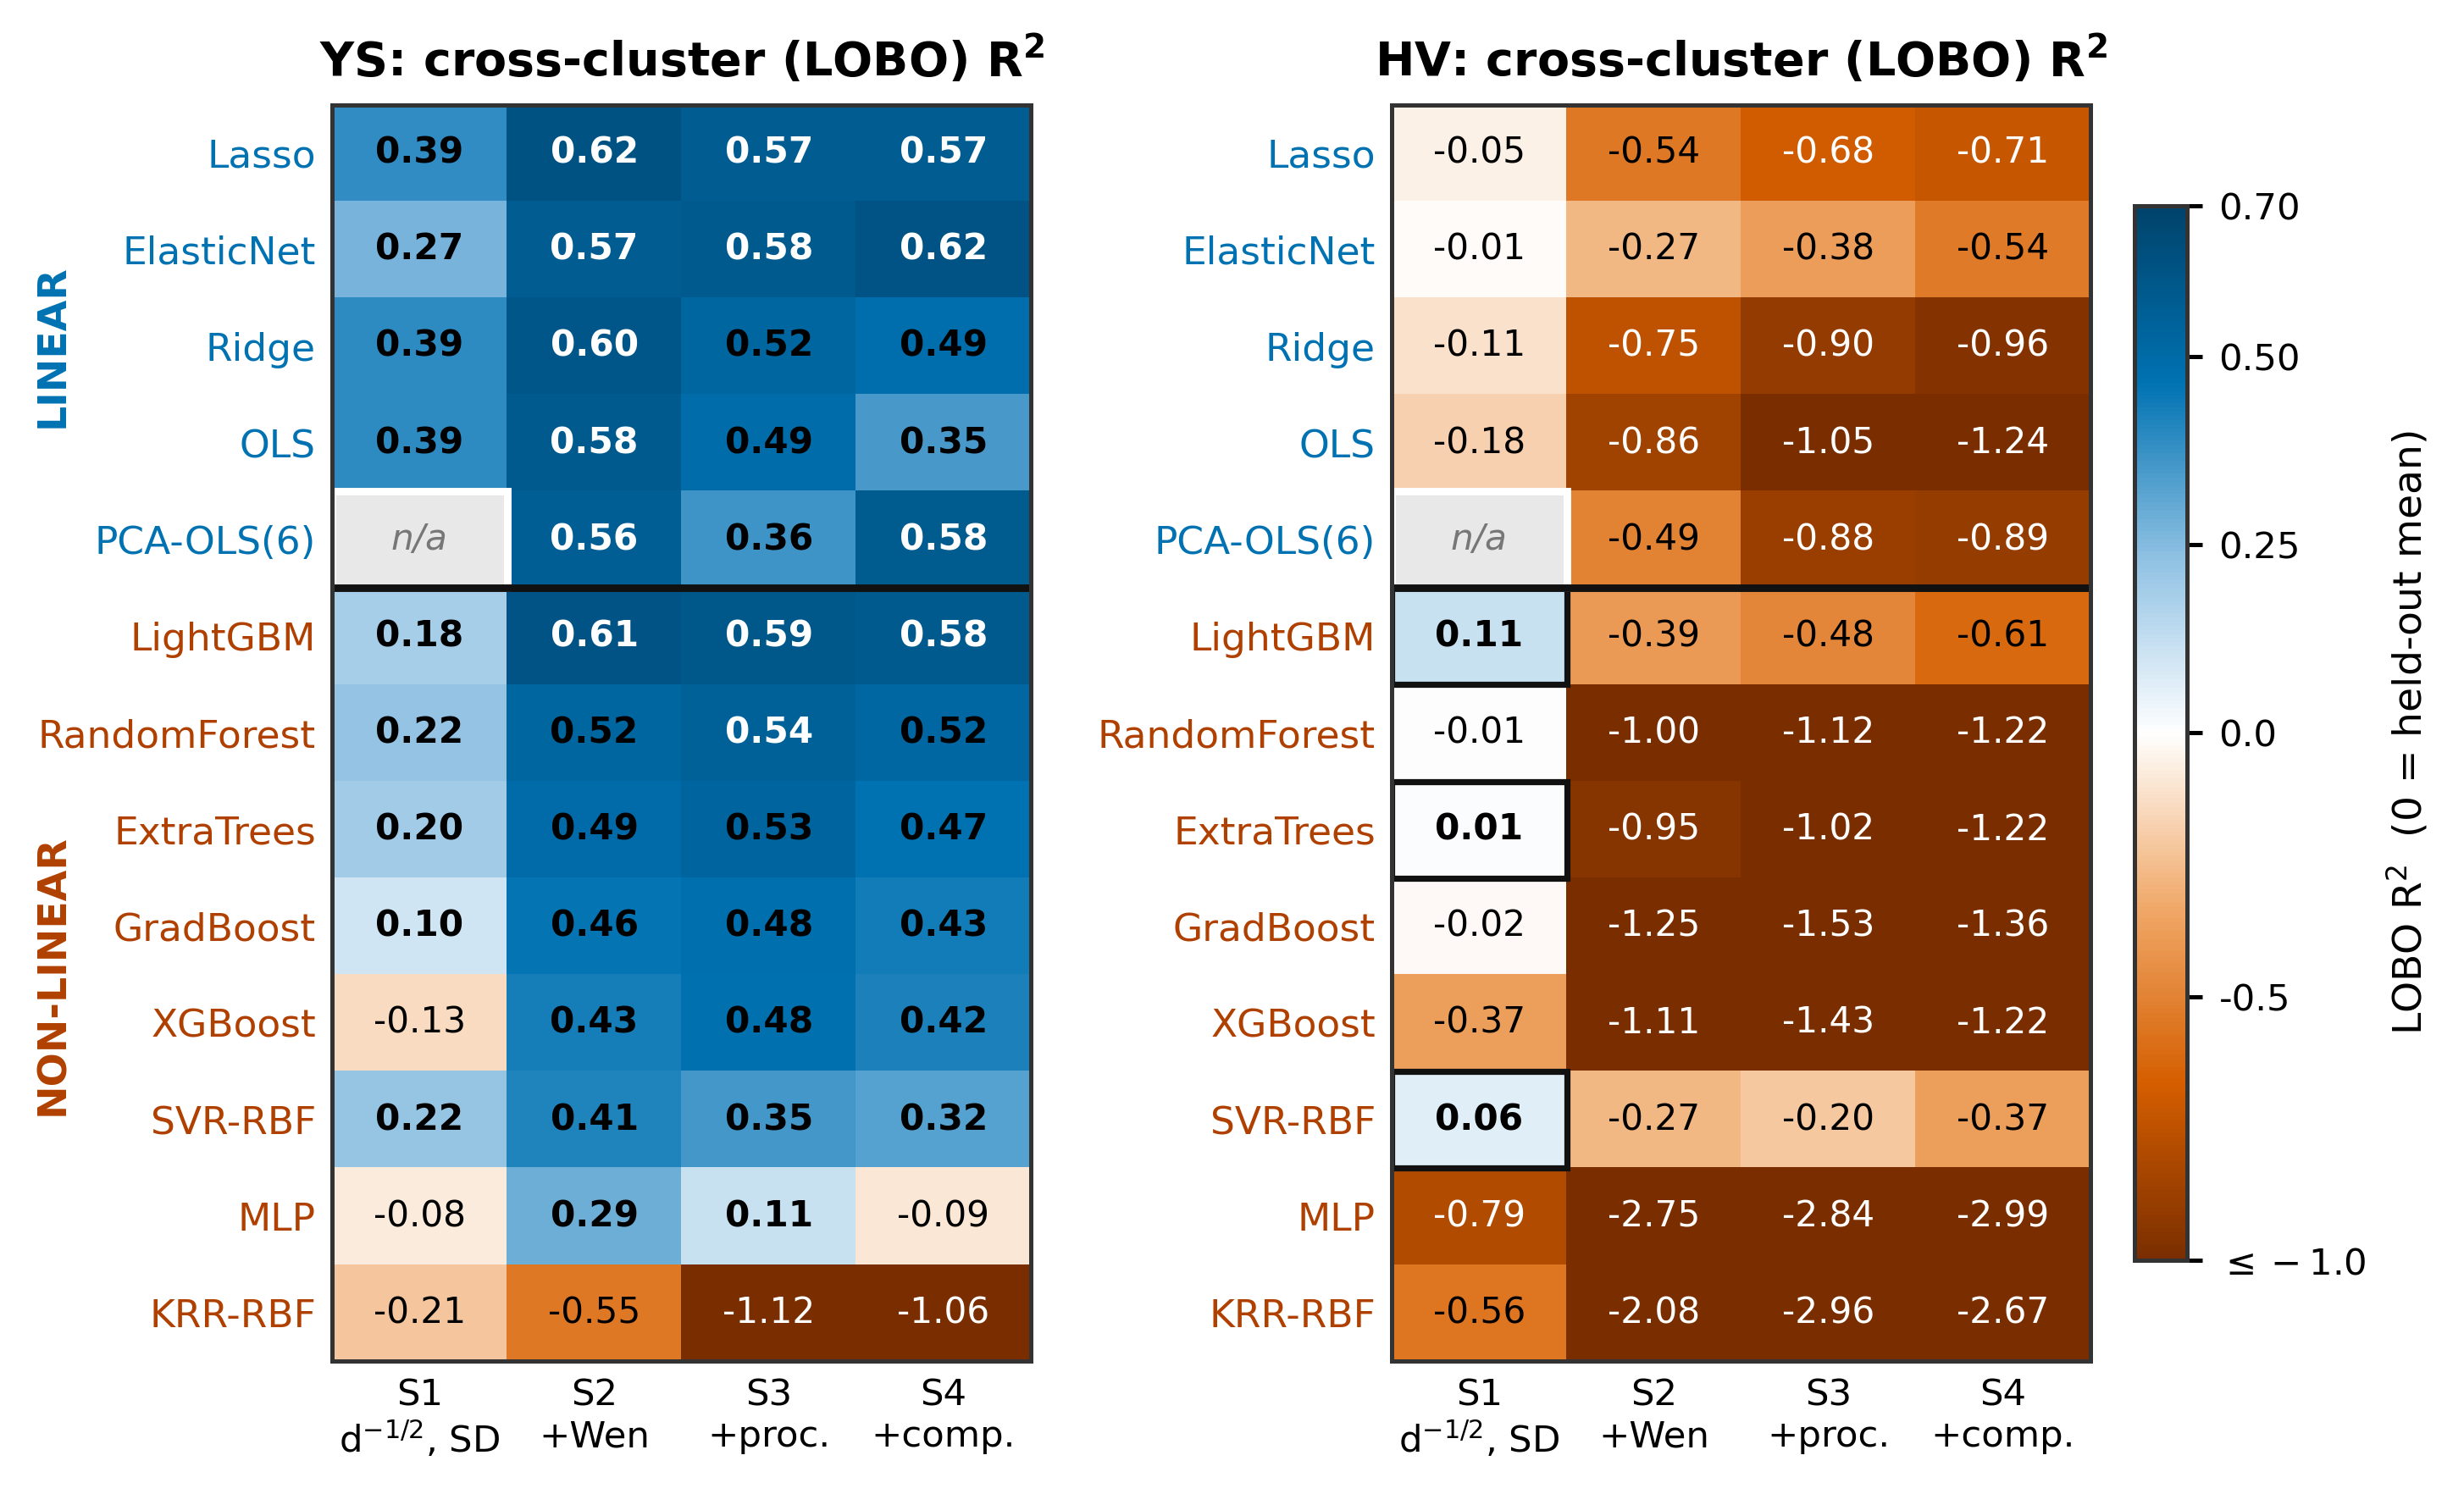
\includegraphics[width=\columnwidth]{fair_comparison_LOBO_heatmap.png}
  \caption{Family~4 matched-input LOBO comparison. For YS, the linear control is competitive with the non-linear estimators. For HV, many descriptor-rich combinations are negative under batch-level validation.}
  \label{fig:fair}
\end{figure}

\subsection{Family 5: \familyfive}

Family~5 searches for compact analytical forms. For YS, the two accuracy-selected PySR equations using composition and processing each reach fixed-form LOO $R^2=0.808$ after their constants are refitted. Their archived mean per-batch LOBO scores are 0.696 and 0.689. A descriptor-based accuracy equation gives LOO/stored-LOBO $R^2=0.765/0.668$, while the descriptor-based elbow equation gives 0.674/0.555. These archived LOBO values are means of fold-wise $R^2$ and are not directly comparable with the pooled $Q^2$ values in Table~\ref{tab:primary}. The descriptor-based accuracy equation contains $\mathrm{SD}_{\mathrm{grain}}/\sqrt{|\Delta S_{\mathrm{mix}}-8.2739|}$. The internal minimum $\Delta S_{\mathrm{mix}}=8.3637$ is only 0.0898 above its pole. The protected square root keeps the expression real on either side, but does not remove the denominator singularity. This equation is therefore unsafe outside the observed descriptor envelope.

All of these PySR values are post-selection scores: the equation structures were chosen from search fronts built with the full dataset. They are not nested estimates of symbolic-regression performance and cannot be ranked directly against the pre-specified models. The complexity--loss front from which they were taken is shown in Fig.~\ref{fig:pysr}. PySR BIC also counts fitted constants but not the cost of searching variables, operators, and structures, so it is not compared with the BIC of the pre-specified linear hierarchy. The SISSO equations have the same selection limitation. Grain-width terms recur across searches and are useful hypotheses, but not independent evidence of a mechanism: all searches use the same 94 records, and $d$ is correlated with $\mathrm{SD}_{\mathrm{grain}}$.

\begin{figure}[t]
  \centering
  
\includegraphics[width=\columnwidth]{fig08_pysr_pareto.png}
  \caption{Family~5 PySR complexity--loss front. Choosing an elbow or accuracy equation after viewing this front places structure selection outside the later constant-refit CV, so the result must be labeled post-selection.}
  \label{fig:pysr}
\end{figure}

Refitting the selected HV structure gives
\begin{equation}
\begin{split}
H_V={}&222.3+84.5\frac{\SI{6.93}{\micro\meter}-d}
                         {\mathrm{SD}_{\mathrm{grain}}}\\
     &-1.005\frac{\Delta H_{\mathrm{mix}}}{t_{\mathrm{hold}}^2}.
\end{split}
\label{eq:hvcorr}
\end{equation}
The three coefficient bootstrap intervals are $[202.9,240.1]$, $[69.4,98.3]$, and $[-1.218,-0.803]$. The corresponding bootstrap means and standard deviations are $221.82\pm9.64$, $84.12\pm7.34$, and $-1.006\pm0.106$; each interval excludes zero, conditional on the selected structure. The full-data fit gives $R^2=0.744$ and RMSE $=16.90$ HV. With the structure fixed and only its constants refitted, 5-fold/LOO/LOBO $R^2=0.725/0.727/0.636$, with RMSE $=17.50/17.46/20.16$ HV. The batch-bootstrap interval for LOBO $R^2$ is $[0.329,0.765]$.

The equation retains useful batch-held-out performance, but its structure was selected after viewing the full-data search fronts. The zero at $d=\SI{6.93}{\micro\meter}$ is not a singularity; the unsafe limits are $\mathrm{SD}_{\mathrm{grain}}=0$ and $t_{\mathrm{hold}}=0$. The observed data remain away from both limits. The two non-constant terms have different provenance risks. Hold time is fixed at 0.5~h for all 35 B-campaign records and takes values of 1, 2, 4, or 8~h in Campaign C, so hold time separates campaign with AUC $=1.000$ and cannot be identified within Campaign B. The combined $\Delta H_{\mathrm{mix}}/t_{\mathrm{hold}}^2$ term also separates campaign strongly (AUC $=0.970$). In contrast, $(6.93-d)/\mathrm{SD}_{\mathrm{grain}}$ is nearly campaign-neutral (AUC $=0.533$). The hold-time term must therefore be treated as a campaign proxy in these data; the grain-width term remains a post-selected, correlated microstructure hypothesis. Testing either term as a mechanism requires a prospectively frozen equation and direct distribution descriptors such as $\mathrm{SD}/d$, lognormal width, or $E[d^{-1/2}]$.

The SISSO comparison also separates numerical safety from predictive accuracy. SISSO Full places $\delta_\mu$ in a denominator and becomes unstable when constituent shear moduli are similar. Removing that term lowers the aggregate literature RMSE from 420.6 to \SI{162.9}{MPa}. The bounded form is numerically safer, but its aggregate $R^2=-1.37$ is still unsuitable for prediction.

Additional symbolic controls give lower or unstable results. An expanded SISSO search reports LOO/LOBO $R^2=0.604/0.350$ when the selected transforms change across folds. A universal-operator EML control gives LOO $R^2=0.321$ at depth one and becomes unstable at greater depth. A recalibrated pure-metal descriptor relation gives LOO $R^2=0.346$. These controls suggest that restricted operators can provide useful inductive bias, but the archived files do not establish that every structure-selection step was nested.

\subsection{Hardness--yield correspondence}

The different YS and HV results motivate a direct comparison of the two properties. Across the 93 paired records, $C_{\mathrm{eff}}=5.13\pm1.36$, corresponding through Eq.~\eqref{eq:napp} to $n_{\mathrm{app}}\approx0.15\pm0.07$ after propagating the reported $C_{\mathrm{eff}}$ summary. The global Spearman correlation is 0.46, although the within-batch correlations range from 0.70 to 0.95. Pooling weakens, but does not reverse, the association; this is aggregation-induced attenuation rather than a strict Simpson paradox. The partial rank correlation after controlling for $d$ is only 0.24.

The archived descriptive relation is $\log C_{\mathrm{eff}}=1.36+0.10\log d-2.06x_V$, with $d$ entered in the fitted numerical units. It is not dimensionally invariant and has not been prospectively validated. Ranking agreement also depends on the cutoff (Fig.~\ref{fig:hvrank}): 2 of the 5 hardest alloys are among the 5 strongest, increasing to 8/10 and 11/20 for broader sets. HV may help rank alloys within a narrow composition and processing window, but the results do not support a single transferable HV-to-YS conversion or identify V as a causal source of the pooled attenuation.

\begin{figure}[t]
  \centering
  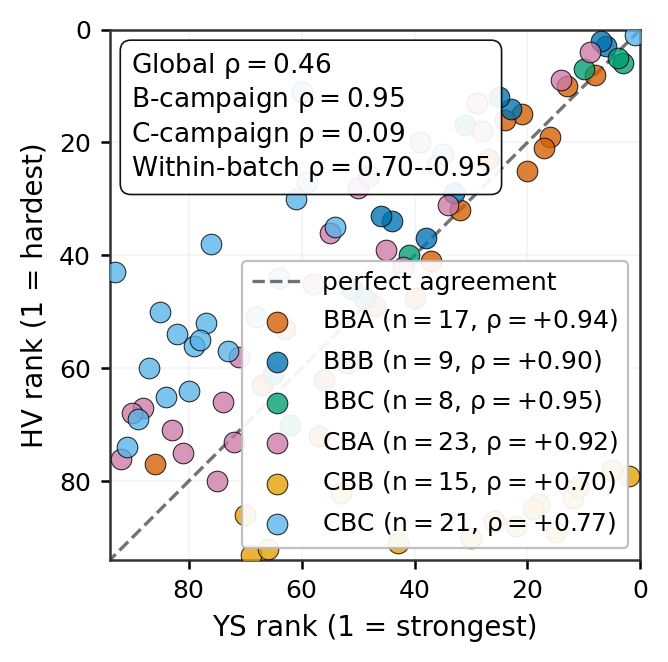
\includegraphics[width=0.90\columnwidth]{fig_hv_ys_rank.png}
  \caption{HV rank versus YS rank by batch. Strong within-batch ordering becomes weaker after batches are pooled because their composition and processing coverage differs.}
  \label{fig:hvrank}
\end{figure}

\subsection{Literature stress test}

The E1 literature set provides a final stress test outside the experimental program. On its 54 direct-strength records, M3 has the lowest RMSE, \SI{149.5}{MPa}, but $R^2=-0.508$. SISSO Robust gives RMSE $=\SI{160.0}{MPa}$ and $R^2=-0.726$, while the small-denominator term in SISSO Full contributes to $R^2=-5.084$. All three models are worse than predicting the E1 mean (Table~\ref{tab:external}). The test is useful for exposing domain sensitivity and unsafe equations, but not for estimating unbiased external performance: E1 mixes sources and test modes and was filtered using outcomes.

The other literature classes give a different appearance because they are not independent direct measurements. On the three E2 values reconstructed from published Hall--Petch fits, M3 and SISSO Robust give descriptive $R^2=0.677$ and 0.849, with RMSE $=49.0$ and \SI{33.5}{MPa}. With $n=3$, these $R^2$ values are not interpretable as generalization estimates. On the 25 E3 hardness-converted proxies, the same models give $R^2=-2.157$ and $-9.642$. Pooling E1--E3 gives M3, SISSO Robust, and SISSO Full $R^2=-0.580$, $-1.373$, and $-14.813$, respectively. Across all 18 stored PySR YS variants, the pooled E1--E3 $R^2$ is also negative; the best is $-0.031$ (RMSE $=\SI{107.4}{MPa}$), and the highlighted descriptor accuracy equation gives $-0.295$ (RMSE $=\SI{120.4}{MPa}$). These pooled values are reported only as numerical stress tests; they do not increase the amount of direct external evidence.

\begin{table}[t]
\centering
\caption{Legacy E1 direct-strength literature stress test. Negative $R^2$ indicates performance worse than predicting the E1 mean.}
\label{tab:external}
\small
\begin{tabular}{lrrr}
\toprule
Model & $R^2$ & RMSE (MPa) & Bias (MPa) \\
\midrule
F3 M3 & $-0.508$ & 149.5 & $-76.6$ \\
F5 SISSO Robust & $-0.726$ & 160.0 & $-61.3$ \\
F5 SISSO Full & $-5.084$ & 300.3 & $+50.0$ \\
\bottomrule
\end{tabular}
\end{table}

\section{Discussion}
\label{sec:discussion}

\subsection{Yield strength across the five families}

The YS results form a clear progression. Family~1 establishes a useful grain-size baseline, but several nearby exponents fit almost equally well. Family~2 shows that the tested SSS and Wen/PCA representations do not provide a transferable improvement with the available approximations. Family~3 supplies the largest verified gain: M3 combines a composition-dependent intercept with a shared Hall--Petch slope, while M15 adds a grain-width interaction and improves LOBO from 0.625 to 0.694. The additive $\mathrm{SD}_{\mathrm{grain}}$ control does not transfer as well, so the result is specific to the interaction. Family~4 reaches similar batch-held-out accuracy with a linear control and a non-linear model, so estimator flexibility is not the source of the gain. Family~5 produces compact equations and further grain-width hypotheses, but its equation search was not nested and its literature performance is negative. M15 is the strongest verified low-complexity YS model when grain-distribution width is measured; M3 remains the simpler choice when only mean grain size is available. Neither is a universal Hall--Petch law.

\subsection{Hardness requires a different model}

The same sequence gives a different result for HV. Mean grain size, physics descriptors, composition, and the tested non-linear models all transfer poorly across batches. Adding $\mathrm{SD}_{\mathrm{grain}}$ linearly improves LOO but worsens LOBO. The post-selected Family~5 fixed form performs well under LOBO after coefficient refitting, but its structure selection was not nested. Its grain-width term is nearly campaign-neutral, whereas its hold-time term closely tracks campaign identity. These terms are worth testing separately, but they do not yet define a hardness law. The variable $C_{\mathrm{eff}}$ and the rank analysis also show why HV should not be treated as a direct substitute for YS across different composition and processing domains.

\subsection{The scientific conclusion depends on validation scale}

The same fitted model can support different conclusions at different validation scales. The clearest examples are for HV: classical Hall--Petch changes from LOO $R^2=0.136$ to LOBO $R^2=-0.077$, LightGBM S1 falls from 0.323 to 0.112, and the legacy tuned XGBoost model falls from 0.729 to 0.574. In Family~2, global PCA gives LOO/LOBO $R^2=0.516/0.441$, whereas fold-contained PCA gives 0.480/0.362, showing how preprocessing and grouping compound. In contrast, M3 changes only modestly from 0.652 to 0.625, and M15 gives 0.694 under both protocols. The Family~5 HV fixed form retains $R^2=0.636$ across batches, but this estimate remains conditional on a structure selected from the full dataset and includes a hold-time term confounded with campaign. LOBO is a useful internal transfer test, but it is not equivalent to deployment because the batches share program-level synthesis, characterization, and design practices.

M15 is therefore the best verified YS model for record-level interpolation and new-batch prediction within the combined experimental program when $\mathrm{SD}_{\mathrm{grain}}$ is available. M3 is a simpler alternative that does not require grain-distribution width. Neither model is a universal Hall--Petch law or a strict test on unseen compositions. Lasso is also useful as a matched predictive control, although it has less direct physical structure. The Family~5 equations remain discovery hypotheses because their structure selection was not nested and their literature evidence is unfavorable. For HV, Eq.~\eqref{eq:hvcorr} is the strongest candidate within the sampled batches, but it should be frozen and tested prospectively before it is treated as a transferable hardness law.

\subsection{Physical interpretation without overreach}

The data support a grain-size baseline for YS together with additional composition- and grain-distribution-associated signals. They do not uniquely attribute those signals to friction stress, solute misfit, boundary chemistry, processing, or hetero-deformation-induced strengthening. The apparent preference for a constant Hall--Petch slope may result from limited identifiability rather than true invariance. $\mathrm{SD}_{\mathrm{grain}}$ appears in M15, the Family~4 feature sets, and several symbolic expressions, but this recurrence is not independent confirmation because the models use the same records and correlated predictors. Raw standard deviation scales with the mean and can also depend on mapped area, grain count, weighting, and segmentation.

YS and HV are not interchangeable labels. Across the 93 paired records, the effective ratio $\mathrm{HV(MPa)}/\sigma_y$ is $5.13\pm1.36$. Strong within-batch rank correlations become weaker when the campaigns are pooled. A single Tabor conversion cannot remove the effects of work hardening, constraint, processing, and campaign structure. Separate models and validation are needed for each property, even though both measurements arise from related plastic-deformation processes.

\subsection{Best practices for physics-informed property ML}

The five families are most useful as a sequence of scientific questions, not as a leaderboard. Family~1 defines a physically interpretable baseline. Family~2 tests whether physics-based descriptors explain the remaining error. Family~3 asks what measured composition and processing add. Family~4 tests estimator flexibility using matched inputs and budgets. Family~5 generates closed-form hypotheses and therefore requires the strictest audit of selection and domain.

For all five families, the validation split must match the proposed use. LOO measures record-level interpolation and must be interpreted alongside the repeated-composition audit. LOBO is needed for claims about a new experimental iteration. Preprocessing, feature selection, hyperparameter tuning, and equation discovery must all occur within that validation boundary. Uncertainty estimates should preserve experimental clusters. Direct measurements should remain separate from values reconstructed from equations or converted from other properties. External sets should be defined before outcomes are inspected and should document composition, processing, grain statistics, phase state, temperature, and test mode. Closed forms also require a singularity audit over both observed and intended deployment domains.

Table~\ref{tab:evidence} maps each claim made in this work onto the evidence that supports it and the interpretation that evidence allows. Mechanistic claims require more than agreement among predictive models. A proposed term should survive alternative parameterizations, dimensional analysis, propagation of measurement uncertainty, and a prospective experiment that varies the proposed cause independently of confounders. For the present grain-width hypothesis, such an experiment should hold mean grain size constant while changing the distribution shape. It should also record complete EBSD distributions and sampling metadata, with the equation frozen before testing.

\begin{table*}[t]
\centering
\caption{Claim--evidence map after grouped-validation and provenance audits.}
\label{tab:evidence}
\small
\begin{tabularx}{\textwidth}{@{}p{3.4cm}p{5.4cm}X@{}}
\toprule
Claim & Evidence & Supported interpretation \\
\midrule
Composition improves YS & M3 LOO/LOBO $R^2=0.652/0.625$ & Supported for record- and batch-level prediction within the present program \\
Grain-width interaction improves YS & Additive SD gives $0.668/0.595$; M15 gives $0.694/0.694$ & Supported as a predictive interaction when SD is measured; mechanism not identified \\
Non-linearity improves YS & Lasso/LightGBM LOBO $0.621/0.615$ & No demonstrated advantage for the tested non-linear model at matched S2 inputs \\
The HV closed form generalizes & Fixed-form LOO/LOBO $0.727/0.636$; post-selected structure & Strongest internal HV candidate; prospective validation is still required \\
Grain-width terms identify a mechanism & Shared data, correlated $d$ and $\mathrm{SD}_{\mathrm{grain}}$, post-selected forms & Testable hypothesis requiring controlled microstructure and prospective validation \\
Models deploy to literature alloys & All evaluated E1 stress-test $R^2<0$; set has mixed modes and outcome-informed curation & No deployment claim and no unbiased external estimate \\
\bottomrule
\end{tabularx}
\end{table*}

\subsection{Limitations and reproducibility}

The analysis includes six batches from two sequential campaigns within one research program. Bayesian-optimization sampling narrows the observed domain, and the composition and processing coverage differs among batches. Exact replicates are limited, processing and composition are not orthogonal, and complete grain-size distributions are reduced to a mean and standard deviation. The literature stress set is not suitable for model selection or an external accuracy claim. A future benchmark should be registered before prediction and should use consistent tensile definitions and complete processing metadata.

The revised repository separates reproducible results from archival, post-selected, and proxy-based results. The scripts \texttt{main2\_validation.py} and \texttt{verify\_sdgrain\_models.py} generate the primary grouped-validation table and the M3/M15 grain-width audit from the prepared descriptor dataset. The standard OLS, information-criterion, and grouped-CV results for M15 are independently reproduced here. Its earlier Bayesian stacking weight and PSIS-LOO comparison remain archival because that probabilistic analysis was not regenerated. Nested ARMOTE-CV and true outer-loop PySR performance also remain unconfirmed until their fold-level generators and predictions are available.

\section{Conclusions}
\label{sec:conclusions}

Physics-informed ML improves materials-property modeling only when physics constrains both the representation and the claim. In the fixed hierarchy of Fig.~1, Family~1 provides the grain-size baseline. Family~2 shows that the tested SSS and Wen/PCA descriptors are redundant or conditional on the campaign. Family~3 gives the clearest verified improvement for YS through a composition-dependent Hall--Petch intercept and a grain-width interaction. Family~4 shows no demonstrated advantage for non-linearity when the inputs are matched. Family~5 produces compact hypotheses, but their selection and transfer remain unresolved.

The key result is the gap between record-level and batch-level validation. M15 gives the strongest verified low-complexity YS performance when $\mathrm{SD}_{\mathrm{grain}}$ is measured, while M3 retains moderate performance without that feature. The tested non-linear estimator does not improve on its linear control at matched inputs. The symbolic HV form performs best across the sampled batches but remains conditional on post-selected structure and a hold-time term confounded with campaign. The practical implication is straightforward. Start with the known physics, test compact descriptors, then add measured composition, processing, and microstructure before increasing estimator complexity. Choose validation groups that match the intended decision. A model should not progress from interpolation to physical interpretation or alloy design without fold-contained selection, cluster-preserving score intervals, outcome-independent external data, and prospective mechanistic tests.

\section*{CRediT authorship contribution statement}
Author-specific CRediT roles will be finalized before submission.

\section*{Declaration of competing interest}
The authors declare that they have no known competing financial interests or personal relationships that could have appeared to influence the work reported in this paper.

\section*{Acknowledgments}
This research was sponsored by the Army Research Laboratory under Cooperative Agreement Number W911NF-22-2-0106. The views and conclusions in this document are those of the authors and should not be interpreted as official policies of the Army Research Laboratory or the US Government. The US Government is authorized to reproduce and distribute reprints for Government Purposes, notwithstanding any copyright notation herein.

We acknowledge Texas A\&M University's Materials Characterization Facility and High Performance Research Computing group for experimental and computational infrastructure.

\section*{Data and code availability}
The project repository contains the raw data, derived descriptors, analysis scripts, result tables, and figure-generation code. The \texttt{paper\_gpt/verified\_results} directory contains the dataset audit, corrected hardness coefficients, evidence-class audit, \texttt{main2\_grouped\_validation.csv}, \texttt{sdgrain\_m15\_validation.csv}, and \texttt{sdgrain\_feature\_audit.csv}. The scripts \texttt{paper\_gpt/main2\_validation.py} and \texttt{paper\_gpt/verify\_sdgrain\_models.py} generate the grouped table and grain-width audits. A versioned public repository identifier and a per-author CRediT statement still need to be added before submission. Nested ARMOTE-CV fold objects and true outer-loop PySR runs are absent, so those results are not treated as confirmatory.

\bibliographystyle{elsarticle-num}
\bibliography{references}

\end{document}
